\documentclass[a4paper]{article}

\usepackage[a4paper, top=8mm, bottom=8mm, left=8mm, right=8mm]{geometry}

\usepackage{polyglossia}
\setdefaultlanguage[babelshorthands=true]{russian}
\setotherlanguage{english}

\usepackage{fontspec}
\setmainfont{FreeSerif}
\newfontfamily{\russianfonttt}[Scale=0.7]{DejaVuSansMono}

\usepackage[tiny, compact]{titlesec}

\usepackage{titling}
\setlength{\droptitle}{-1cm}
\pretitle{\begin{center}\begin{bfseries}\Large}
\posttitle{\par\end{bfseries}\end{center}}
\preauthor{\begin{center}\normalsize}
\postauthor{\par\end{center}\vspace{-1.8cm}}

\usepackage{hyperref}
\usepackage{bookmark}
\usepackage{csquotes}
\usepackage{float} 
\usepackage{booktabs}
\usepackage{graphicx}


\title{Архиватор на базе алгоритма Хаффмана}

\author{Кочанов Андрей Иванович}


\date{}

\begin{document}

\maketitle

\begin{flushright}
    Группа: \emph{25.Б43-мм}

    Кафедра: \emph{системного программирования}

    Научный руководитель: \emph{Литвинов Юрий Викторович}

    Номер семестра практики: \emph{2}
\end{flushright} 

\section{Введение}

Алгоритм Хаффмана — один из наиболее известных алгоритмов сжатия данных без потерь, основанный на понятии <<префиксных кодов>> — битовых последовательностей, обладающих тем свойством, что код каждого символа не является префиксом кода никакого другого символа. Это позволяет при прочтении битовой последовательности однозначно восстанавливать символы по их битовым кодам. Работа носит учебный характер и направлена на освоение приёмов работы с динамическими структурами данных, битовыми операциями и модульным проектированием на языке C, что делает её полезной для освоения низкоуровневых возможностей языка C.

\section{Постановка задачи}

\textbf{Целью работы является} получение практического опыта разработки программного обеспечения на примере задачи реализации архиватора на базе алгоритма Хаффмана, а также измерение эффективности сжатия и скорость работы.

\textbf{Для достижения цели требуется решить следующие задачи:}
\begin{enumerate}
    \item Выполнить обзор существующих реализаций алгоритма Хаффмана.
    \item Спроектировать архитектуру консольного приложения.
    \item Реализовать консольное приложение.
    \item Выполнить тестирование и эксперименты.
\end{enumerate}

\section{Обзор}

\textbf{Алгоритм Хаффмана} предложен Д.~Хаффманом в 1952~году~[1].
Идея состоит в построении бинарного дерева, листья которого
соответствуют символам алфавита, а путь от корня до листа задаёт
префиксный код: часто встречающимся символам достаются короткие
коды, редким~--- длинные. Алгоритм жадно объединяет два узла
с наименьшими частотами, поэтому дерево строится за
$O(n \log n)$ при использовании очереди с приоритетом. Алгоритм Хаффмана гарантирует построение кода с минимально возможной средней длиной для заданного распределения частот при условии, что каждый символ кодируется отдельным кодовым словом~[2].

\textbf{Канонические коды Хаффмана.}
В классическом алгоритме Хаффмана декодеру передают таблицу частот символов, и он самостоятельно построит по ней точно такое же дерево, по которому символы были закодированы.
Канонические коды оптимальнее передачи таблицы частот. Передача таблицы частот требует сохранения пар «символ-частота», а также заставляет декодер заново строить дерево Хаффмана, выполняя те же $O(n \log n)$ операций. Канонические же коды позволяют передать только длины кодовых слов. Для алфавита из 256 символов это дает уменьшение заголовка с нескольких килобайт до сотни байт, а декодер восстанавливает коды за линейное время без построения дерева.
Сами коды восстанавливаются по строго определённому правилу. Сначала символы сортируются по возрастанию длины кода, а при равной длине — по возрастанию значения самого символа. Код минимальной длины инициализируется нулями в соответствующем количестве бит. Каждый следующий код той же длины получается прибавлением единицы к предыдущему. При переходе к коду большей длины он дополняется нулями справа на разницу длин.
Такие коды применяются, например, в форматах DEFLATE, JPEG и MP3.

В качестве ориентиров рассмотрены открытые реализации на языке C:

\begin{itemize}
    \item SmnTin/huffman-archiver [3]: реализация на C с каноническими кодами Хаффмана, оптимизированная для больших файлов; демонстрирует высокую пропускную способность.
    \item MichaelDipperstein/huffman [4]: простая ANSI~C реализация с классическими и каноническими кодами.
\end{itemize}

\textbf{Вывод из обзора}
Анализ этих реализаций позволил
выделить общие архитектурные решения. Из huffman-archiver SmnTin~[3]
заимствована идея буферизации битового вывода: биты накапливаются в байте
и записываются блоками, что ускоряет работу с потоком. Из учебной
реализации MichaelDipperstein~[4]~---~подход к построению дерева через
очередь с приоритетом и сериализации таблицы частот в заголовок.

\section{Описание предлагаемого решения}

\subsection{Архитектура}

\begin{itemize}
    \item \texttt{bitReader}, \texttt{bitWriter}~--- побитовое чтение
    и запись с внутренним байтовым буфером;
    \item \texttt{bitIO}~--- сериализация целых чисел
    в формате little-endian;
    \item \texttt{minHeap}~--- очередь с приоритетом на бинарной куче;
    \item \texttt{huffmanTree}~--- узел дерева и построение дерева
    по таблице частот;
    \item \texttt{prefCodeTable}~--- ленивая таблица префиксных кодов;
    \item \texttt{huffman}~--- публичный интерфейс функций сжатия и разжатия файлов
\end{itemize}

Код разделён на модули по принципу единственной ответственности. Такое разделение позволяет тестировать компоненты изолированно и локализует изменения: замена структуры данных или формата заголовка затрагивает один модуль, не распространяясь на остальные. Альтернатива в виде монолитного файла дала бы небольшой выигрыш по скорости за счёт инлайнинга, но существенно усложнила бы отладку и покрытие тестами.

\subsection{Технологии}

\begin{itemize}
    \item Язык C99, компилятор GCC 16 (также собирается Clang и MSVC).
    \item Система сборки: CMake ≥ 3.25.
    %4.4.3
    \item Статический анализ: clang-format (WebKit), clang-tidy.
    \item CI через GitHub Actions: сборка, проверка форматирования, линтинг, интеграционные тесты на Linux.
\end{itemize}

\subsection{Технические детали}

\begin{itemize}
    \item \textbf{Инкапсуляция.} Определения структур вынесены в~\texttt{.c}-файлы,
    в заголовках оставлены только непрозрачные объявления.
    Доступ к полям~--- исключительно через функции-аксессоры.
    Это соответствует принципу единственной ответственности
    и исключает связывание модулей через детали реализации.

    \item \textbf{Таблица кодов.} Код символа вычисляется
    при первом обращении к нему и кэшируется в таблице. Повторные
    обращения к тому же символу не пересчитывают код: при первом
    появлении символа стоимость~---~$O(n)$ ($n$~---~длина кода),
    при последующих~---~$O(1)$. Это даёт выигрыш на файлах
    с большим числом повторяющихся символов, так как дорогостоящее вычисление кода (подъём от листа к корню) выполняется всего один раз для каждого уникального символа.

    \item \textbf{Заголовок.} Формат файла: 8~байт исходного размера,
    2~байта числа уникальных символов, далее для каждого символа~---
    1~байт значения и 8~байт частоты; после заголовка~---~битовый
    поток.

    \item \textbf{Особые случаи.} Пустой файл~---~записывается только
    заголовок. Файл с единственным уникальным символом~---~ни одного
    бита данных, при распаковке символ повторяется нужное число раз.

    \item \textbf{Коды ошибок.} Вместо одного значения~$-1$ используется
    перечисление \texttt{HuffmanResult} с разными кодами для
    «не удалось открыть входной файл», «не удалось создать выходной
    файл», «ошибка памяти», «ошибка чтения», «ошибка записи»,
    «некорректный формат». Это позволяет вызывающей стороне
    различать ситуации без парсинга \texttt{stderr}.
\end{itemize}

\section{Эксперименты}

Для оценки эффективности алгоритма были поставлены эксперименты,
измеряющие степень сжатия, время сжатия и время распаковки
на разных типах и размерах данных. Использованы пять категорий:
повторяющиеся текстовые (repeat, .txt), обычные текстовые (text, .txt),
случайные байты (random, .bin), уже сжатые архивы (archive, .zip)
и изображения в формате JPEG (photo, .jpg). В качестве <<обычных текстовых>> данных использовался отрывок из романа Г.~Мелвилла <<Моби Дик>> на английском языке. 
Для каждой категории~---~10~прогонов с расчётом математического
ожидания ($\mu$) и среднеквадратичного отклонения ($\sigma$).

\begin{itemize}
    \item Компилятор: gcc версии 16.2.1
    \item Флаги компиляции: -O3 -DNDEBUG
    \item Процессор: AMD Ryzen 5 3500U, 1{,}4--3{,}7 ГГц
    \item Оперативная память: DDR4, 8 ГиБ
    \item Частота шины памяти: 1333 МГц
    \item Операционная система: EndeavourOS, ядро Linux~7.x
\end{itemize}

\begin{table}[H]
\centering
\small
\caption{Экономия размера, \% от исходного размера}
\label{tab:ratio}
\begin{tabular}{lrrrrr}
\toprule
Тип & 1 КБ & 10 КБ & 100 КБ & 1 МБ & 5 МБ \\
\midrule
repeat  & 98.14 & 99.81 & 99.98 & 99.99 & 99.99 \\
text    & 10.64 & 41.86 & 44.95 & 45.26  & 45.29  \\
archive & $-216.02$ & 26.37 & 41.47 & 52.83 & 54.07 \\
random  & $-222.66$ & $-22.56$ & $-2.26$ & $-0.22$ & $-0.04$ \\
photo   & $-190.24$ & $-21.24$ & $-1.99$ & 8.65 & 0.01 \\
\bottomrule
\end{tabular}
\end{table}

\begin{table}[H]
\centering
\small
\caption{Время сжатия, мс ($\mu \pm \sigma$, 10 прогонов)}
\label{tab:compress}
\begin{tabular}{lrrrrr}
\toprule
Тип & 1 КБ & 10 КБ & 100 КБ & 1 МБ & 5 МБ \\
\midrule
repeat  & $1.63 \pm 0.45$ & $1.44 \pm 0.28$ & $2.56 \pm 0.81$ & $8.76 \pm 1.36$ & $37.52 \pm 3.39$ \\
text    & $1.85 \pm 0.49$ & $2.66 \pm 0.72$ & $11.21 \pm 3.43$ & $77.78 \pm 4.48$ & $372.82 \pm 6.79$ \\
archive & $1.67 \pm 0.18$ & $2.69 \pm 0.77$ & $9.16 \pm 1.72$ & $50.92 \pm 3.26$ & $240.96 \pm 14.47$ \\
random  & $2.14 \pm 0.58$ & $3.41 \pm 0.87$ & $15.97 \pm 4.35$ & $120.68 \pm 3.90$ & $579.23 \pm 6.58$ \\
photo   & $1.76 \pm 0.33$ & $5.06 \pm 1.28$ & $15.25 \pm 3.53$ & $122.82 \pm 4.81$ & $625.19 \pm 19.84$ \\
\bottomrule
\end{tabular}
\end{table}

\begin{table}[H]
\centering
\small
\caption{Время распаковки, мс ($\mu \pm \sigma$, 10 прогонов)}
\label{tab:decompress}
\begin{tabular}{lrrrrr}
\toprule
Тип & 1 КБ & 10 КБ & 100 КБ & 1 МБ & 5 МБ \\
\midrule
repeat  & $1.58 \pm 0.31$ & $1.30 \pm 0.12$ & $2.77 \pm 0.88$ & $11.91 \pm 3.03$ & $50.85 \pm 6.63$ \\
text    & $1.89 \pm 0.48$ & $2.95 \pm 0.94$ & $10.45 \pm 1.79$ & $84.39 \pm 4.48$ & $404.91 \pm 6.63$ \\
archive & $1.87 \pm 0.45$ & $3.19 \pm 0.57$ & $9.48 \pm 2.41$ & $55.37 \pm 3.69$ & $251.26 \pm 7.26$ \\
random  & $1.84 \pm 0.30$ & $3.12 \pm 0.73$ & $17.48 \pm 4.05$ & $133.38 \pm 4.94$ & $638.79 \pm 6.81$ \\
photo   & $1.56 \pm 0.11$ & $5.05 \pm 1.38$ & $15.87 \pm 2.06$ & $136.32 \pm 4.51$ & $672.20 \pm 12.27$ \\
\bottomrule
\end{tabular}
\end{table}

\begin{figure}[H]
    \centering
    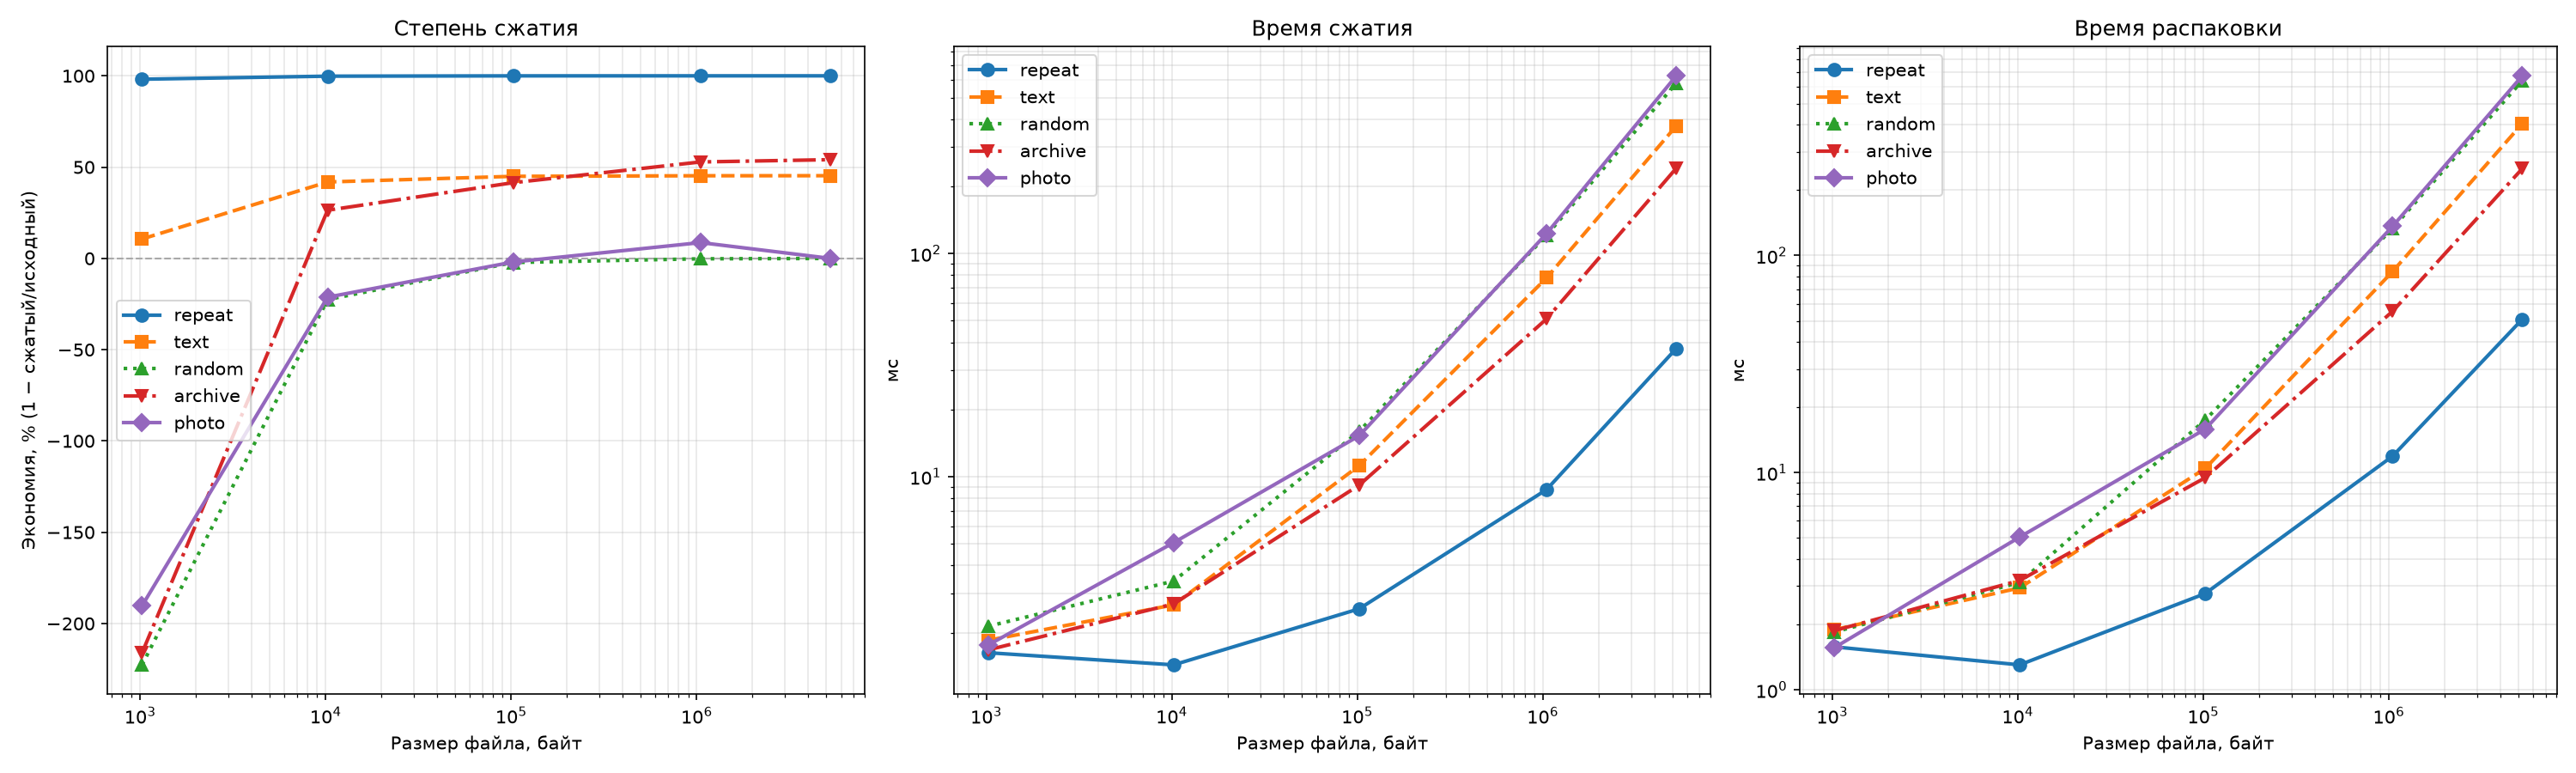
\includegraphics[width=\textwidth]{graphs.png}
    \caption{Зависимость степени сжатия и времени работы от размера файла}
    \label{fig:experiment}
\end{figure}

\subsection{Выводы из результатов эксперимента}

\begin{itemize}
    \item Эффективность сжатия определяется энтропией входных данных
    и размером алфавита. Однородные данные (\texttt{repeat}) сжимаются
    почти идеально: при одном уникальном символе код занимает~0~бит,
    сжатый файл для всех размеров равен~19~байтам (только заголовок),
    экономия~---~от~98.1\% на~1~КБ до~99.99\% на~5~МБ. Текст
    сжимается на~42--45\% для размеров от~100~КБ; на~1~КБ~---~
    всего~10.6\% из-за накладных расходов на заголовок
    ($8 + 2 + 9k$~байт, где~$k$~---~число уникальных символов).
    Архивы ZIP дают~26--54\% экономии, поскольку в наборе данных
    они содержат текст и служебные заголовки. (См. Таблицу 1)

    \item На случайных данных и JPEG-изображениях алгоритм
    неэффективен: на~1~КБ размер вырастает на~190--222\%
    из-за доминирующего заголовка, а на~5~МБ практически
    не меняется ($-0.04\%$ для \texttt{random}, $+0.01\%$
    для~\texttt{photo}). Это ожидаемо: обе категории уже имеют
    высокую энтропию, и префиксный код не может их сжать. (См. Таблицу 1)

    \item Время работы асимптотически линейно зависит
    от размера входного файла ($O(n)$): и сжатие, и распаковка
    выполняются за один проход по данным. При увеличении размера
    с~1~КБ до~5~МБ (в~5000~раз) время сжатия выросло
    в~20--350~раз в зависимости от типа данных: наименьший рост
    у~\texttt{repeat} ($\approx 23\times$), наибольший~---~
    у~случайных и сжатых данных (\texttt{photo}: $\approx 355\times$). (См. Рисунок 1)

    \item Разброс времени ($\sigma$) для крупных файлов
    составляет~1--5\% от~$\mu$, что говорит о стабильности
    измерений. На~1--10~КБ стабильность ниже: относительный
    вклад операций открытия файла, выделения памяти и системных
    вызовов становится заметнее. (См. Таблицу 2 и Таблицу 3)

    \item Самыми медленными оказались случайные данные
    и фотографии: из-за~256 уникальных символов средняя длина
    кода приближается к~8~битам, поэтому на каждый байт входа
    приходится выполнять почти столько же побитовых операций,
    сколько занимал сам байт, и экономии не происходит. (См. Таблицу 2 и Таблицу 3)
\end{itemize}


\section{Заключение}

В ходе выполнения работы получены следующие результаты:

\begin{itemize}
    \item изучена теория префиксных кодов и алгоритма Хаффмана,
    включая канонические коды;
    \item реализован модульный консольный архиватор на C
    с инкапсулированными структурами данных, ленивой таблицей
    префиксных кодов и явной обработкой ошибок;
    \item построена система интеграционных тестов, покрывающая
    полный цикл «сжатие~---~распаковка» для текстовых,
    вырожденных и пустых файлов;
    \item проведены эксперименты по измерению степени сжатия
    и времени работы на данных пяти типов; сформулированы
    выводы о применимости алгоритма.
\end{itemize}

Репозиторий/ссылка на пуллреквест: \url{https://github.com/Andrew-Kochanov/archiverHuffman}.

Техническая документация: \url{https://github.com/Andrew-Kochanov/archiverHuffman/blob/main/README.md}.

\section*{Список литературы}

\begin{enumerate}
    \item Huffman D.~A. A Method for the Construction of Minimum-Redundancy
    Codes // Proceedings of the IRE. — 1952. — Vol.~40, No.~9. — P.~1098--1101.

    \item Cormen T.~H., Leiserson C.~E., Rivest R.~L., Stein C.
    Introduction to Algorithms. --- 3rd ed. --- MIT Press, 2009. --- Ch.~16.3.

    \item SmnTin. huffman-archiver [Электронный ресурс]. — URL:
    \url{https://github.com/SmnTin/huffman-archiver}
    (дата обращения: 08.10.2026).

    \item MichaelDipperstein. huffman: Huffman code discussion and
    implementation [Электронный ресурс]. — URL:
    \url{https://github.com/MichaelDipperstein/huffman}
    (дата обращения: 08.10.2026).
\end{enumerate}


\end{document}


исправь мой отчет в соответствии с комментариями преподавателя(изменения делай только по ним):
1) в тексте должны быть ссылки на каждую таблицу и рисунок
2) написать на какие именно обычных данных мы делаи эксперименты
3) в технических деталях в пункте про заголовок    
4) в технических деталях в пункте про таблицу написать, почему она дает выигрыш в файлах с большим количеством повторяющихся символов
5) в обзоре в пункте про канонические коды написать: по какому "строго определнному правилу"  можно постановить коды по длиннам(кратко изложить основную идею); написать больше относительно чего становится файл, если передавать дерево целиком, и еще же не обязательно передавать дерево, можно передать таблицу частот(обработай этот случай)


в конце напиши, что конкретно исправил.